\section{Using the Milestones Project for Statistical Historiography}\label{sec:historiography}
\epigraph{Vision is the art of seeing things invisible.}{Johnathan Swift, 1711}

\begin{comment}
\begin{itemize*}
  \item comparisons of graphical innovations by field (e.g. physical sciences vs. social sciences), in terms of content and form
  \item extract themes and relationships between content areas
\end{itemize*}
\end{comment}

\subsection{Statistical historiography}\label{sec:stathist}
We use the term ``statistical historiography,'' to refer to the use of statistical and graphical methods to explore, study and describe historical problems and questions.%
\footnote{As far as we know, the initial expression of this idea appeared in a paper by \citet{Rubin:1943} discussing various ways in which statistical methods could be applied to historical topics.  These included: the use of sampling methods to test historical theories; statistical distributions applied to historical data; and, the use of time series graphs with smoothed curves to study historical trends. More recently, many examples of the application of these ideas to statistical topics can be found in \citet{Stigler:1986,Stigler:1999}, as well as our own papers on the history of data visualization, cited \emph{inter alia}.}
This topic has a delightful self-referential quality when applied to the history of data visualization itself, since we have often found ourselves using modern methods of statistical analysis and graphics to study the development of ideas in this area. As in the quotation from Swift above, one goal is to make previously hidden aspects of this history visible.

At the same time, our examination of some of the most impressive graphic works of the past sometimes left us awe-struck by their exquisite beauty and visual design.%
\footnote{Some examples are: Charles Joseph Minard's famous depiction of Napoleon's March on Moscow \citep{Friendly:02:Minard}, Francis Galton's detailed study of weather patterns in Europe \citep[see:][]{Friendly:2008:golden}, and Andr{\'e}-Michel Guerry's \citep[Plate 17]{Guerry:1864} semi-graphic table depicting the relations of occurrence of crimes to a wide variety of social and demographic factors \citep[see:][]{Friendly:2007:guerry}.}
On more than one occasion when looking at these elegant presentations, we wondered whether there wasn't something lost with the advent of modern software. While we can now analyze massive data sets, and generate a multitude of graphics with a simple mouse click, we still feel that designing a truly effective visual display of information requires thought and manual intervention.

For this reason, it is often quite instructive to attempt to re-create or even re-vision a graphic work from the past \citep{Friendly:02:Minard}. 
We can learn from this undertaking an appreciation for the insight and hard labor of our graphic heros, and can sometimes better understand 
or improve on their designs by a process we call ``understanding through reproduction,'' another facet of statistical historiography.

We illustrate this approach with an analysis of a graph from \citet{Playfair:1821}
shown in \figref{fig:playfair-wheat1}, in some ways a tour-de-force of
early graphic presentation. In this graph, Playfair used three parallel time
series in different forms
to show the price of wheat (bar chart), weekly wages (line graph), and reigning monarch (bars at the top)
over a $\sim$250 year span from 1565 to 1820. His graphic goal was rhetorical: he wished to
argue that workers had become better off in the most recent years. Surely this must be counted
among the best early data graphics.

%% one figure
\begin{figure}[htb]
  \centering
  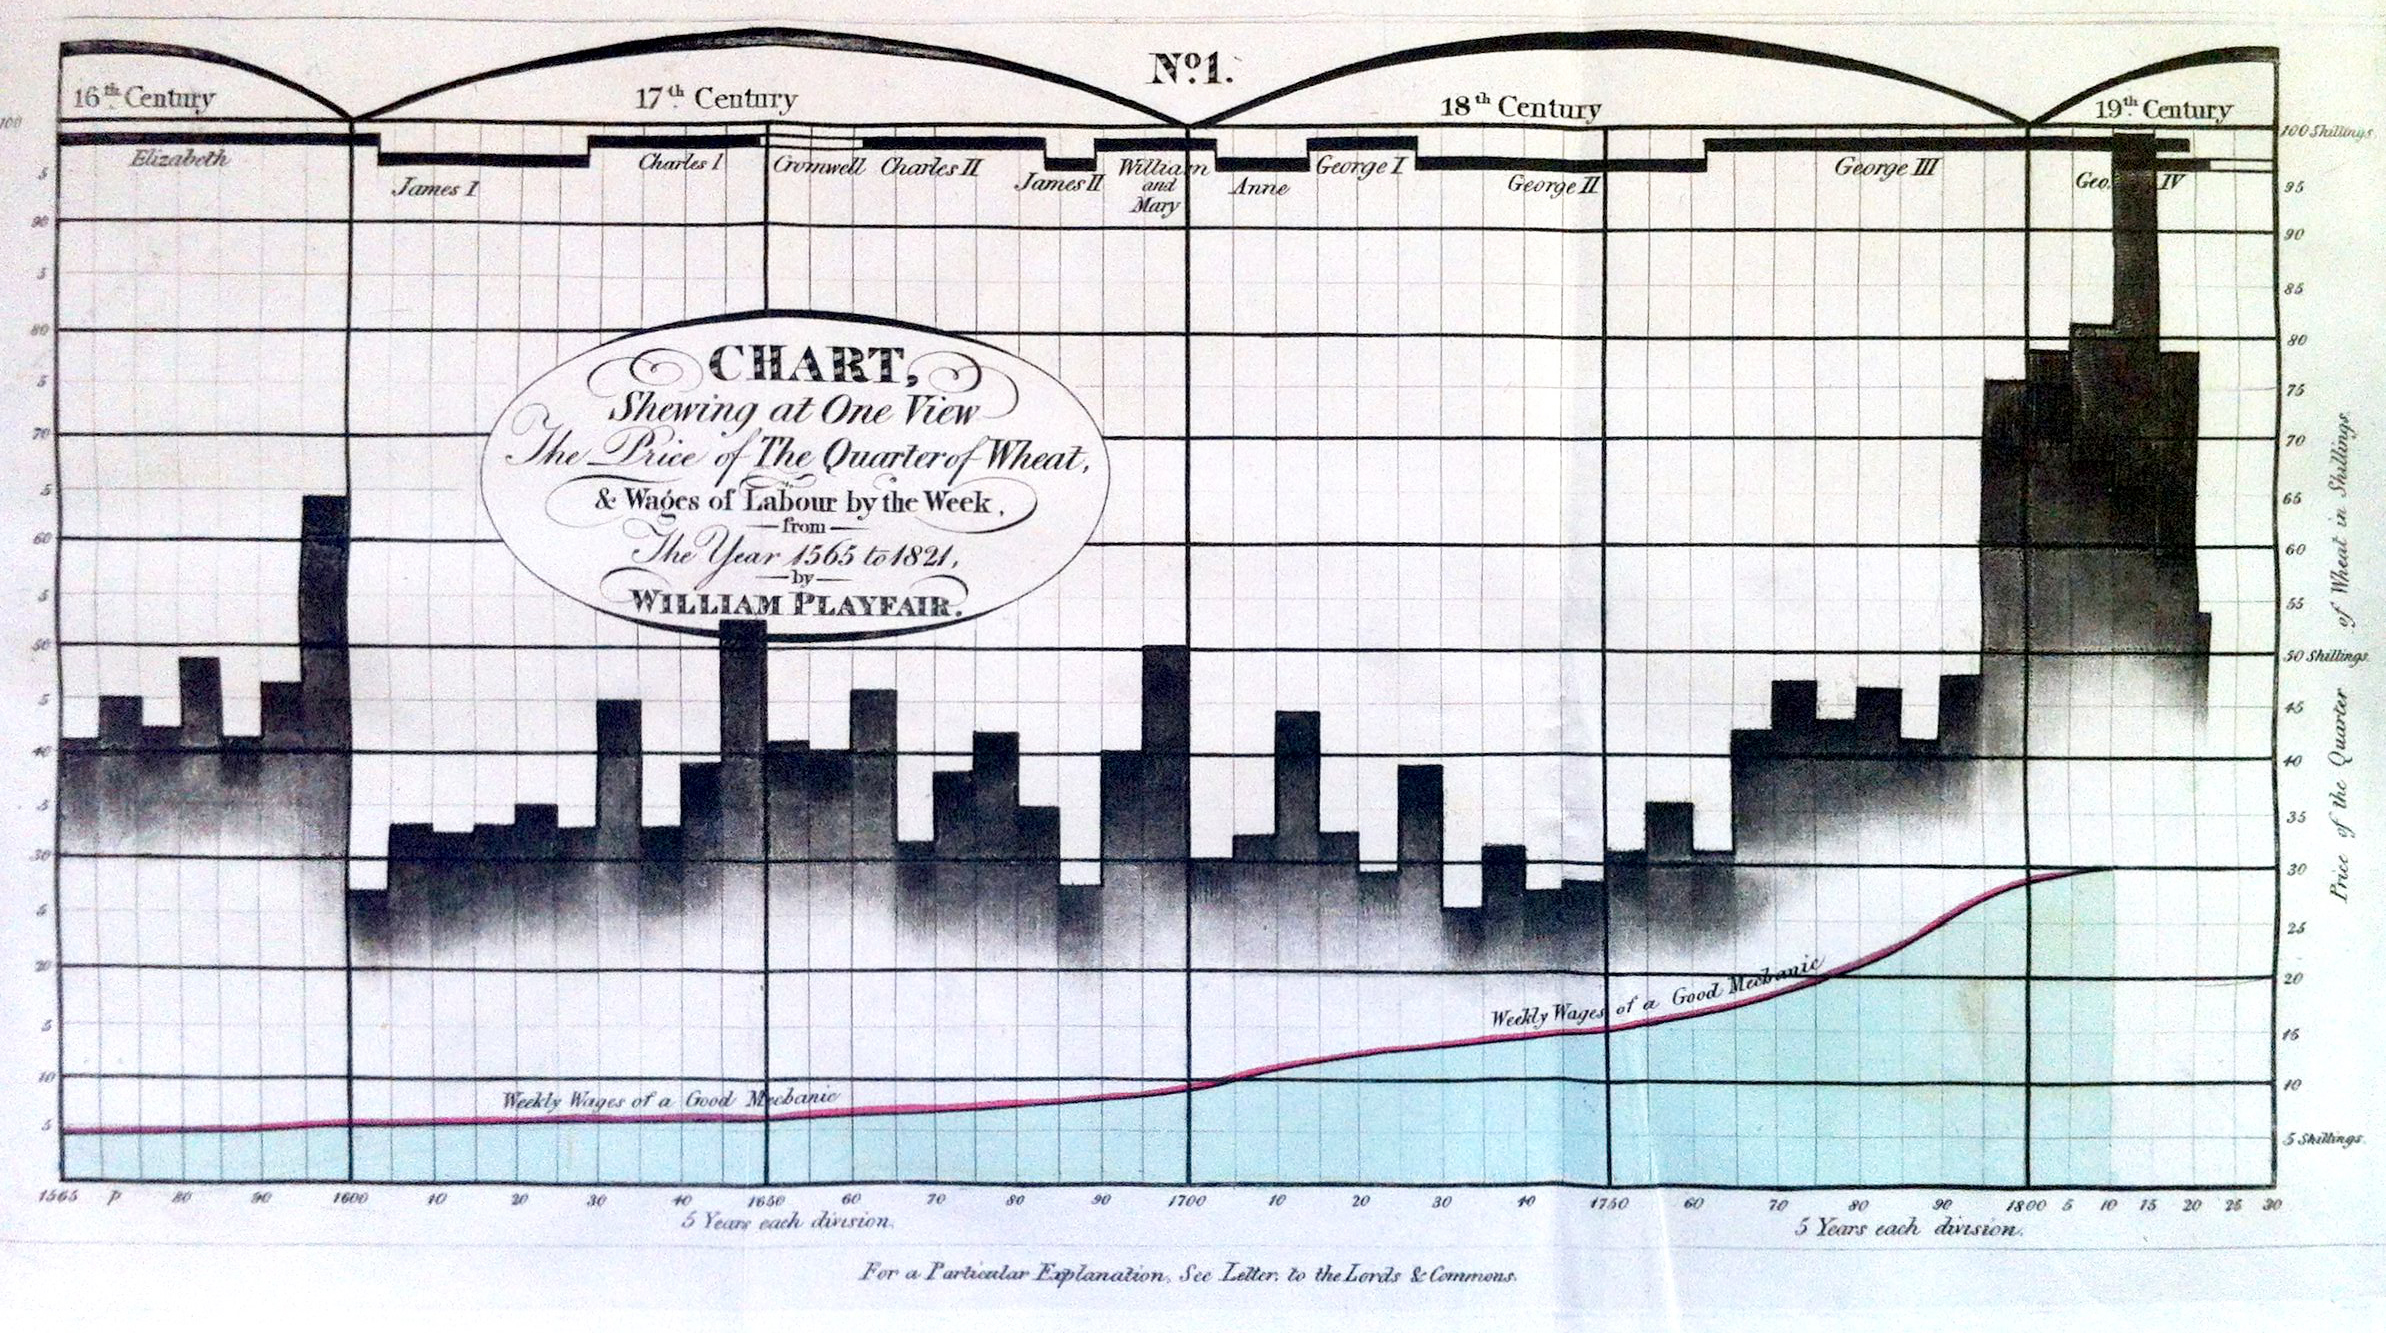
\includegraphics[width=\textwidth]{fig/Playfair1821b}
  \caption{William Playfair's 1821 time series graph of prices, wages, and ruling monarch
  over a 250 year period.
  \emph{Source}: \cite{Playfair:1821}, image from Stephen Stigler.}%
  \label{fig:playfair-wheat1}
\end{figure}

Yet, as we have argued elsewhere \citep{FriendlyDenis:05:scat}, this graph is both sinful
and a communication failure for Playfair's purpose.  It is sinful because the use of separate $y$ axes for
wages (left axis, range: 0--100) and prices (right axis, range: 0--30) on different scales
provides the opportunity to tell very different stories simply by re-scaling one or both
axes.

%% one figure
\begin{figure}[!htb]
  \centering
  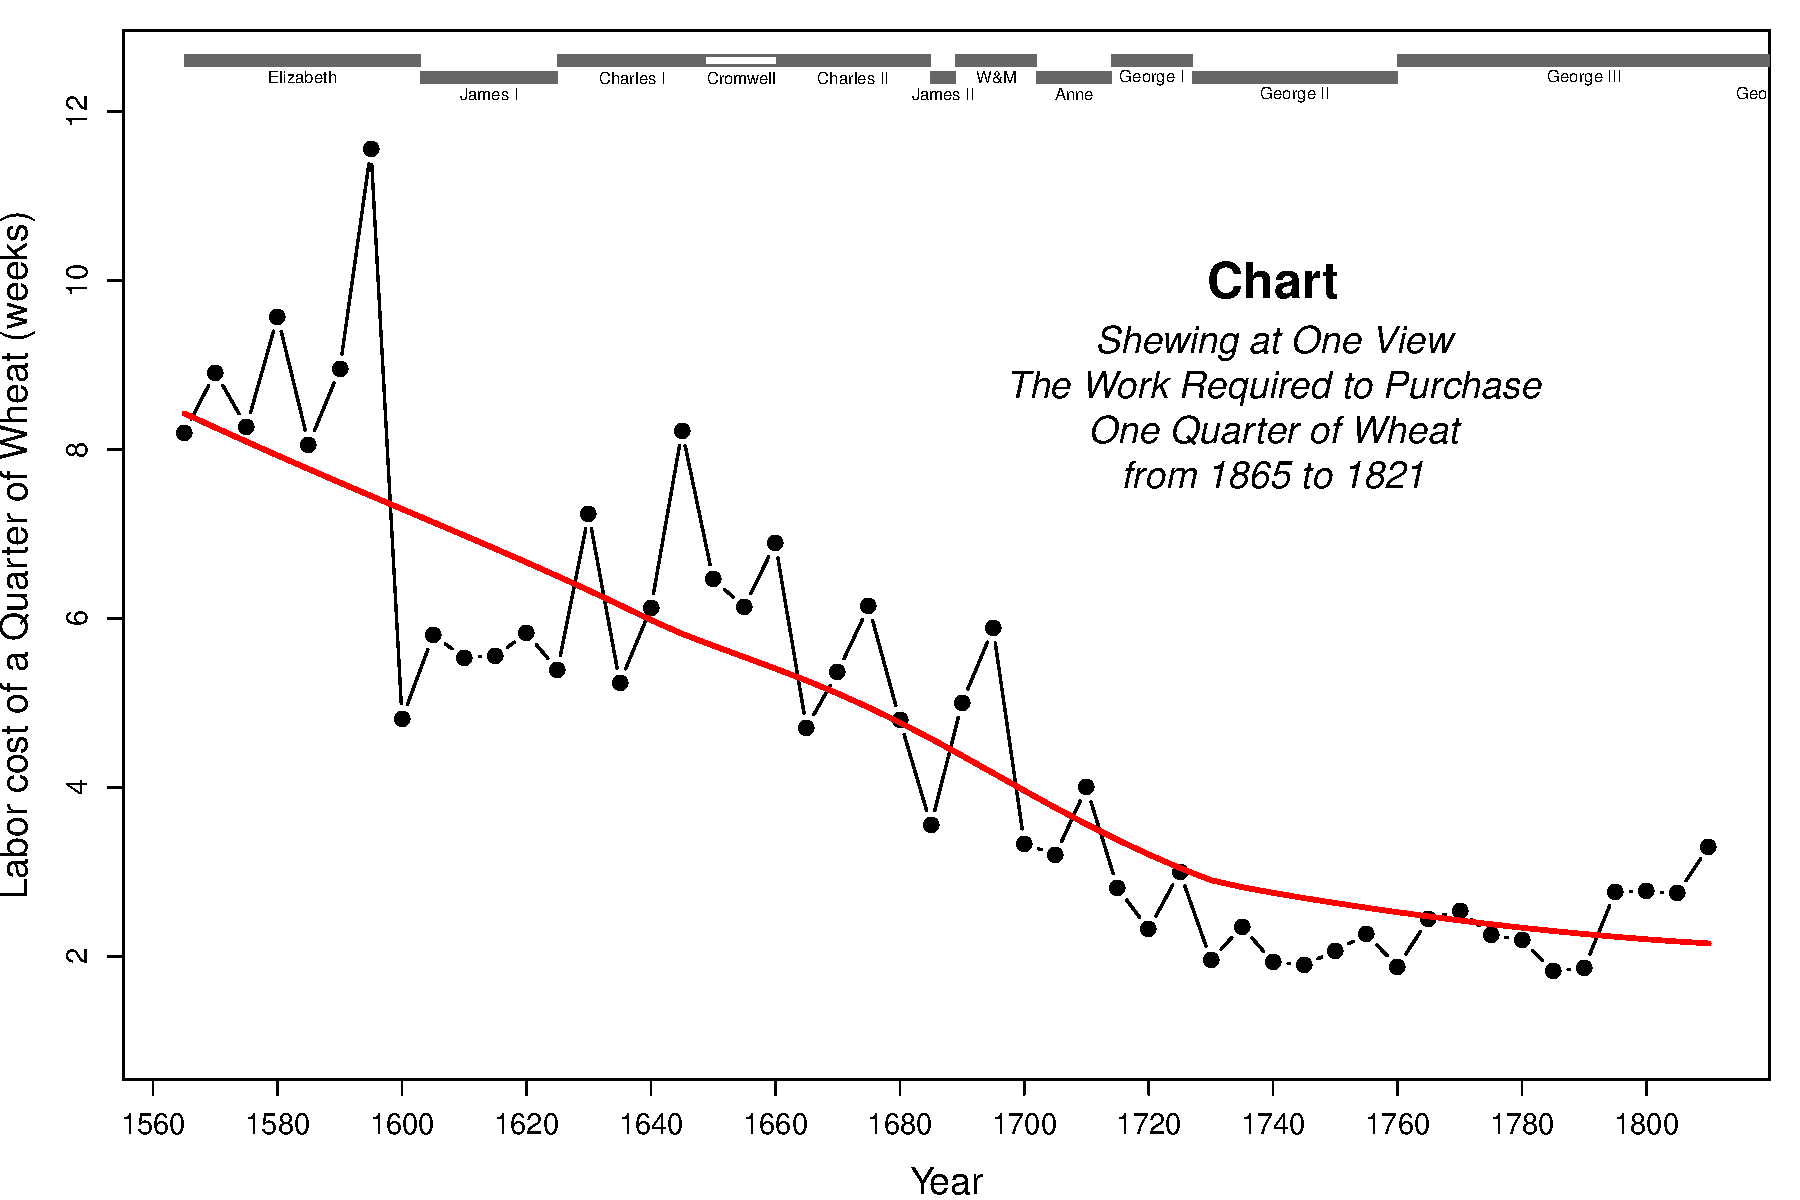
\includegraphics[width=.9\textwidth,clip]{fig/wheat2}
  \caption{Redrawn version of Playfair's time series graph
  showing the ratio of price of wheat to wages,
  together with a loess smoothed curve.}
  \label{fig:wheat1}
\end{figure}

It is also a graphic failure because the visual impression that wages increased relative to prices
toward the right end is at best indirect and is obscured by the large fluctuations in prices of wheat.
What Playfair might have done to show the relation directly, is to plot the \emph{ratio} of price to wages,
representing the labor cost of a unit of wheat, as we have done in \figref{fig:wheat1}.%
\footnote{
Playfair's data and this re-creation can be found in the \texttt{R} package HistData \citep{HistData}
as \texttt{example(Wheat)}.
}
Adding a non-parametric (loess) smoothed curve to the line plot makes Playfair's message directly apparent;
it also shows that the reduction in the amount of labor required to purchase one unit of week in fact
levels off in the last 40 years. As well, it highlights that something quite unusual happened around 1600.


However, in order to conduct such statistical historiography, there is one principal requirement: \textbf{data}. The Milestones Project database is the repository of all the information we have so far recorded, and modern database tools allow the possibility of simple or complex queries, limited only by the available information.%
\footnote{It should be noted that, beyond the basics of recording milestones items, images and references, inputting the other meta-data (content and form categories, keywords, etc.) is highly labor-intensive. Thanks are due to many research assistants and graduate students who have and continue to work on the Milestones Project, including Dan Denis, Matt Dubins, Yvonne Lai, Avi Lipton, and Carolina Patryluk.}
In related work, we have collected and disseminated data sets of historical interest on a variety of topics in statistics and data visualization, for instance via the \texttt{R} packages HistData \citep{HistData} and Guerry \citep{Guerry}. These can be considered another source for data, pictures, and stories related to statistical historiography, and understanding through reproduction. This is the essence of the motto on the \url{datavis.ca} web site: \emph{Looking back, going forward}.

In the subsections below, we describe a few applications of these ideas using the Milestones Project database and case studies that arose from this work. There is an interesting interplay between such historical analyses and these data collections. Some studies called for us to find and incorporate new data sources, such as our paper \citep{Friendly:2007:guerry} on Guerry's \emph{Moral statistics of France} and the Guerry package, to which we added Angeville's extensive 1836 data on social and economic characteristics of France. In other cases, our analyses suggested new or different ways to visualize historical data.

\subsection{Milestone authors: lifespan}\label{sec:lifespan}
As noted earlier, we record information relevant to the contributors of milestones events in an author table in the database. For most of these individuals, internet and biographical searches allowed us to determine the dates and places of their birth and death.

One simple question that can be posed using this information is how long did these contributors live? As illustrated earlier (see \figref{fig:timespan}), Joseph Priestley was the first to develop the idea of using a graphic representation to show the lifespan of famous men. His ``charts of biography'' did this in a particularly evocative form, representing each person by a line segment whose length was defined by the individual's lifespan, and then grouped by occupational category.

These ``timespan'' charts tell an interesting story, but they do not provide an answer to the question of how long, in general, these individuals lived.  However, with the author table from the Milestones Project, it is a simple matter to calculate lifespan, and obtain a direct answer to this query. \figref{fig:lifespan} shows one display of this information, using a combined density plot and rug plot, similar to the one used in \figref{fig:mileyears4}.

\begin{figure}[!htb]
  \centering
  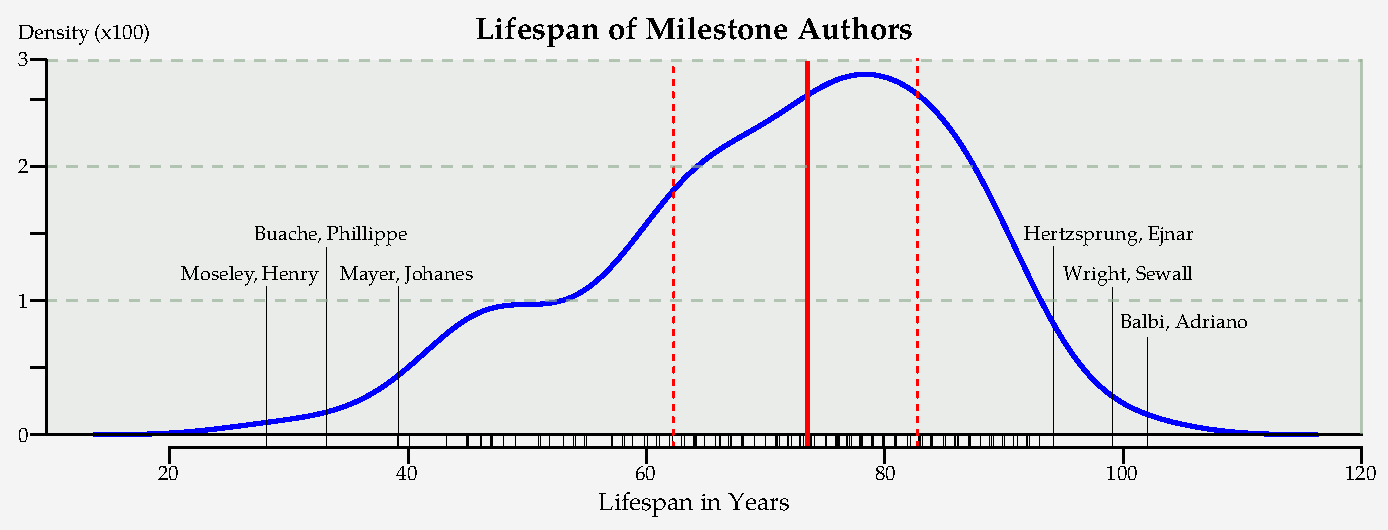
\includegraphics[width=\textwidth,clip]{fig/lifespan3}
  \caption{Density plot of the lifespan of the 172 authors in the Milestones Project database who were born after 1500 and for whom lifespan can be determined. Individual observations are shown by a (jittered) rug plot, and the three extremes on each end are identified by name.  The red vertical lines show the quartiles of the distribution.}
  \label{fig:lifespan}
\end{figure}

Several features of this plot deserve comment, and also invite further inquiry: Most notable is that, by and large, milestones authors generally lived to a ripe old age--- the median lifespan is 73.0, but the density plot peaks at around 79. This contrasts with a detailed study on famous people between 2400 BC to 1880 AD by David de la Croix and Omar Licandro (\url{http://www.fcs.edu.uy/archivos/BCU_clebrities.pdf}).  In their research, it was found that the typical lifespan fluctuated around a mean of 61 years for four millennia, and only gradually reached 69 toward the end of their sample. Such a discrepancy between the two studies might warrant further investigation; for instance, by classifying the individuals into occupational, locational, or otherwise more delineated groups, and looking for trends.

Another interesting feature that becomes apparent in this graphic is the noticeable bump in the distribution around 45 years. This occurrence calls for some attempt at further explanation. We don't pursue this here, but again note that such graphs often suggest further analyses (breakdowns by region or time period), or cry out for the collection of more data.

Finally, although \figref{fig:lifespan} is just a summary graph, we have labeled a few extreme observations on each end, which may relate to telling parts of the story of the history of data visualization.  Among these, Henry Moselely, who is known for the discovery of atomic number from a graphical display, died the youngest, as a consequence of serving in the British Army during World War I. But, we were surprised to see the noted and prolific French cartographer Phillippe Buache, and the German physicist and astronomer Johann Tobias Mayer, show up in positions two and three.  On the other end, we were delighted to see that Adriano Balbi, a Venetian geographer and early collaborator of Andr{\'e}-Michel Guerry \citep{BalbiGuerry:1829} had the longest lifespan, just exceeding the population geneticist, Sewall Wright, who invented path analysis and the path diagram around 1920.  By incorporating these details, the visualization is able to reveal narratives that otherwise would have been concealed.

\subsection{Milestone authors: geography}\label{sec:geography}
The Milestones Project web site provides an initial page showing an interactive timeline of the events in this history as a visual overview (\figref{fig:mileyears4}). A long-term goal has been to provide other views of this history and other tools for searching and exploring the database. With recent technological developments, it became evident to us that one such method would be through the use of geographical data.

So far, the primary geographic information we have encoded in the database refers to the birth and death place of the milestone authors. This is an imperfect representation, as these locations may not accurately represent the author's primary residence.  For instance, Charles Joseph Minard was born in Dijon, and died in Bordeaux, but all of his work was done in Paris while he worked at the {\'E}cole Nationale des Ponts et Chauss{\'e}es. Nevertheless, a geographic view of the available information is potentially useful. In this regard, we used the Google geocoding tools to provide latitude and longitude for the locations listed in the author table.  Using this and the R package googleVis \citep{googleVis}, we created the interactive map shown in \figref{fig:authormap}.

\begin{figure}[!htb]
  \centering
  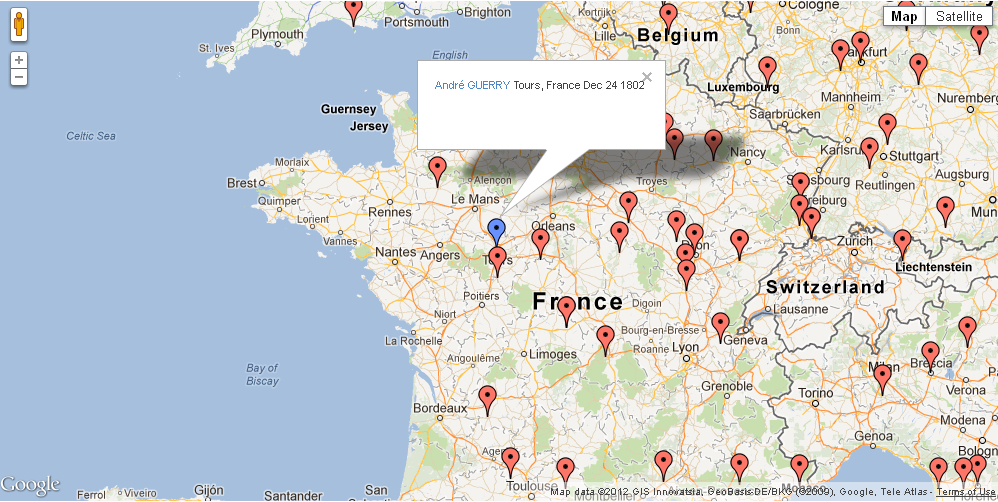
\includegraphics[width=\textwidth,clip]{fig/authormap}
  \caption{Birth places of 188 milestone authors, shown on an interactive Google map, centred on France. Each geographic marker is linked to an author query on the \texttt{datavis.ca} web site that lists the contributions by that individual.}
  \label{fig:authormap}
\end{figure}

Like other instances of Google Maps, this graphic can be panned and zoomed using mouse controls. The place markers display tool tips when hovered over and, when clicked, link to a search page that details all of the Milestone items that are related to that author. This interesting visualization will soon be revealed on the Milestones Project website, with future work planned to incorporate other types of data in addition to the birth and death locations.

\subsection{Milestones: themes and trends}\label{sec:themes}
The records in the Milestones Project database also feature various text fields for each logged event. These include a brief item tag, a full description of the event, and relevant keywords, as well as categorical codes for the content (Subject), and form  (Aspect) of the item. Treating this information as ``data'' allows us and others to study themes and trends in these developments.  Modern methods of text mining and data visualization can provide insights into this history not available through other means.

As one simple illustration of this approach, \figref{fig:milecats4} shows two mosaic displays%
\footnote{Mosaic displays show the frequencies in cells of a cross-classified table by the area of each tile.  The tiles are shaded according to departure from a null
model of no-association, using blue for cells with frequencies substantially greater than chance, and red for cells with frequencies that are lower than expected.}
that explore the relationships among Epoch, Subject, and Aspect. The left panel shows changes in the distributions of milestone events by Subject over time.  It can readily be seen that while most of the milestone innovations up to the end of the \Cent{18} were about the physical world (astronomy, geodetic measurement, weather, etc.), this trend changed in the \Cent{19}, where there was a large shift toward problems that related to human populations (e.g., pertaining to mortality, births, disease, crime). Beginning in the early 1900s, the pattern changes again, with advances in mathematics and statistics becoming the dominating force.

\begin{figure}[!htb]
  \centering
  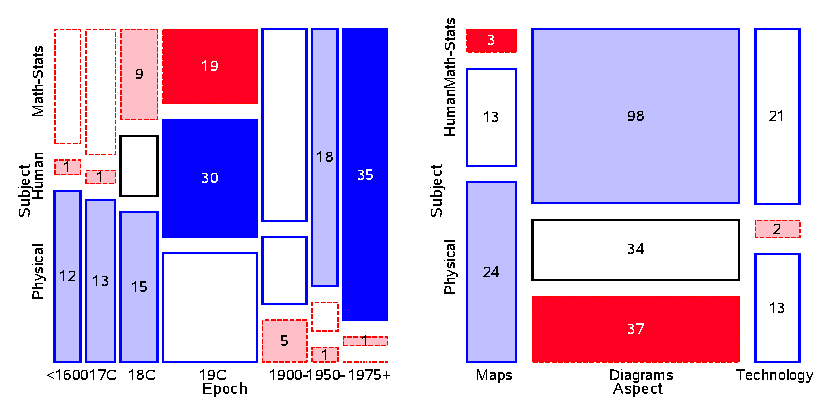
\includegraphics[width=\textwidth,clip]{fig/milecats4}
  \caption{Mosaic displays for milestone items, classified by Epoch, Subject and Aspect. Left: mosaic for the marginal table showing differences in Subject across Epochs; Right: mosaic for the marginal table showing differences in Subject across Aspect. Numbers in the tiles give the number of milestone items.}
  \label{fig:milecats4}
\end{figure}

The right panel shows the association between Subject and Aspect, pooled over Epoch. As is not surprising, maps and other cartographical representations were most often used to show data of the physical world, while graphs and diagrams were most often associated with mathematical and statistical subjects.

Other statistical graphs and analyses could be used to explore these and other relationships in more detail. The key to this is of course the existence and availability of data--- in this case reflected by the coding of graphical milestones in our database.
